\section{Slot Composition}

\begin{enumerate}
\item 
We show here $2$ examples of mixing images, by using some slots from one image and some from other. 

\item The first $2$ images ($Image_1$ and $Image_2$ respectively) in \autoref{fig:composition1} and \autoref{fig:composition2}
are the images used for \verb|mixing| and the rightmost on is produced by mixing \verb|slots|, from the \verb|encodings| of first $2$ and then decoding them.

\item 
For reference, \autoref{fig:slot_images1} and \autoref{fig:slot_images2}  shows respectively the masks generated from the $7$ slots for $Image_1$ and $Image_2$

\item \autoref{fig:generated_iamges} shows other generated images after using K-Means clustering to cluster slots and then randomly picking one slot from each cluster to generate the image.

\end{enumerate}

\begin{figure}[hbt!]
    \centering
    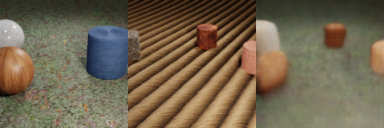
\includegraphics[width=0.8\textwidth]{images/mixed_1.png} 
    \caption{Slot mixing example 1}
    \label{fig:composition1}
\end{figure}

\begin{figure}[hbt!]
    \centering
    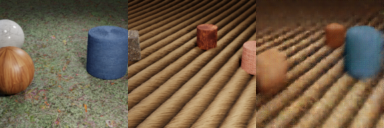
\includegraphics[width=0.8\textwidth]{images/mixed_2.png} 
    \caption{Slot mixing example 2}
    \label{fig:composition2}
\end{figure}

\begin{figure}[hbt!]
    \centering
    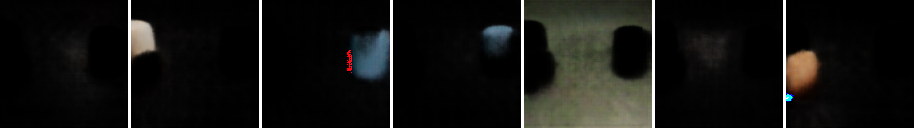
\includegraphics[width=0.8\textwidth]{images/slots_images_1.png} 
    \caption{Slot-wise images for $Image_1$}
    \label{fig:slot_images1}
\end{figure}

\begin{figure}[hbt!]
    \centering
    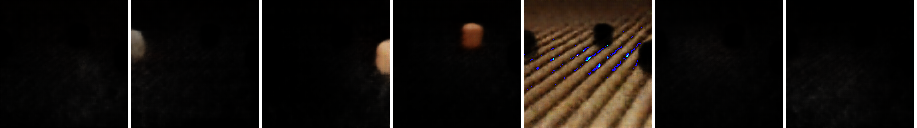
\includegraphics[width=0.8\textwidth]{images/slots_images_2.png} 
    \caption{Slot-wise images for $Image_2$}
    \label{fig:slot_images2}
\end{figure}


\begin{figure}[hbt!]
    \centering
    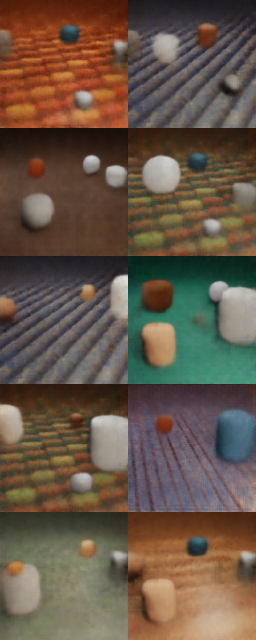
\includegraphics[width=0.5\textwidth]{images/generated_iamges.png} 
    \caption{Generated images by randomly picking Slots after K-means clustering}
    \label{fig:generated_iamges}
\end{figure}